\subsection{Summary}
\label{sub:model_summary}

To alleviate these problems we propose a different model structure. Our model inherits many features from agent-based simulation models but replaces the contacts between moving particles by contacts between individuals who work, go to school, live in a household and enjoy leisure activities. The structure of the model is depicted in Figure~\ref{fig:model_graph}.

\begin{figure}[!ht]
    \centering
    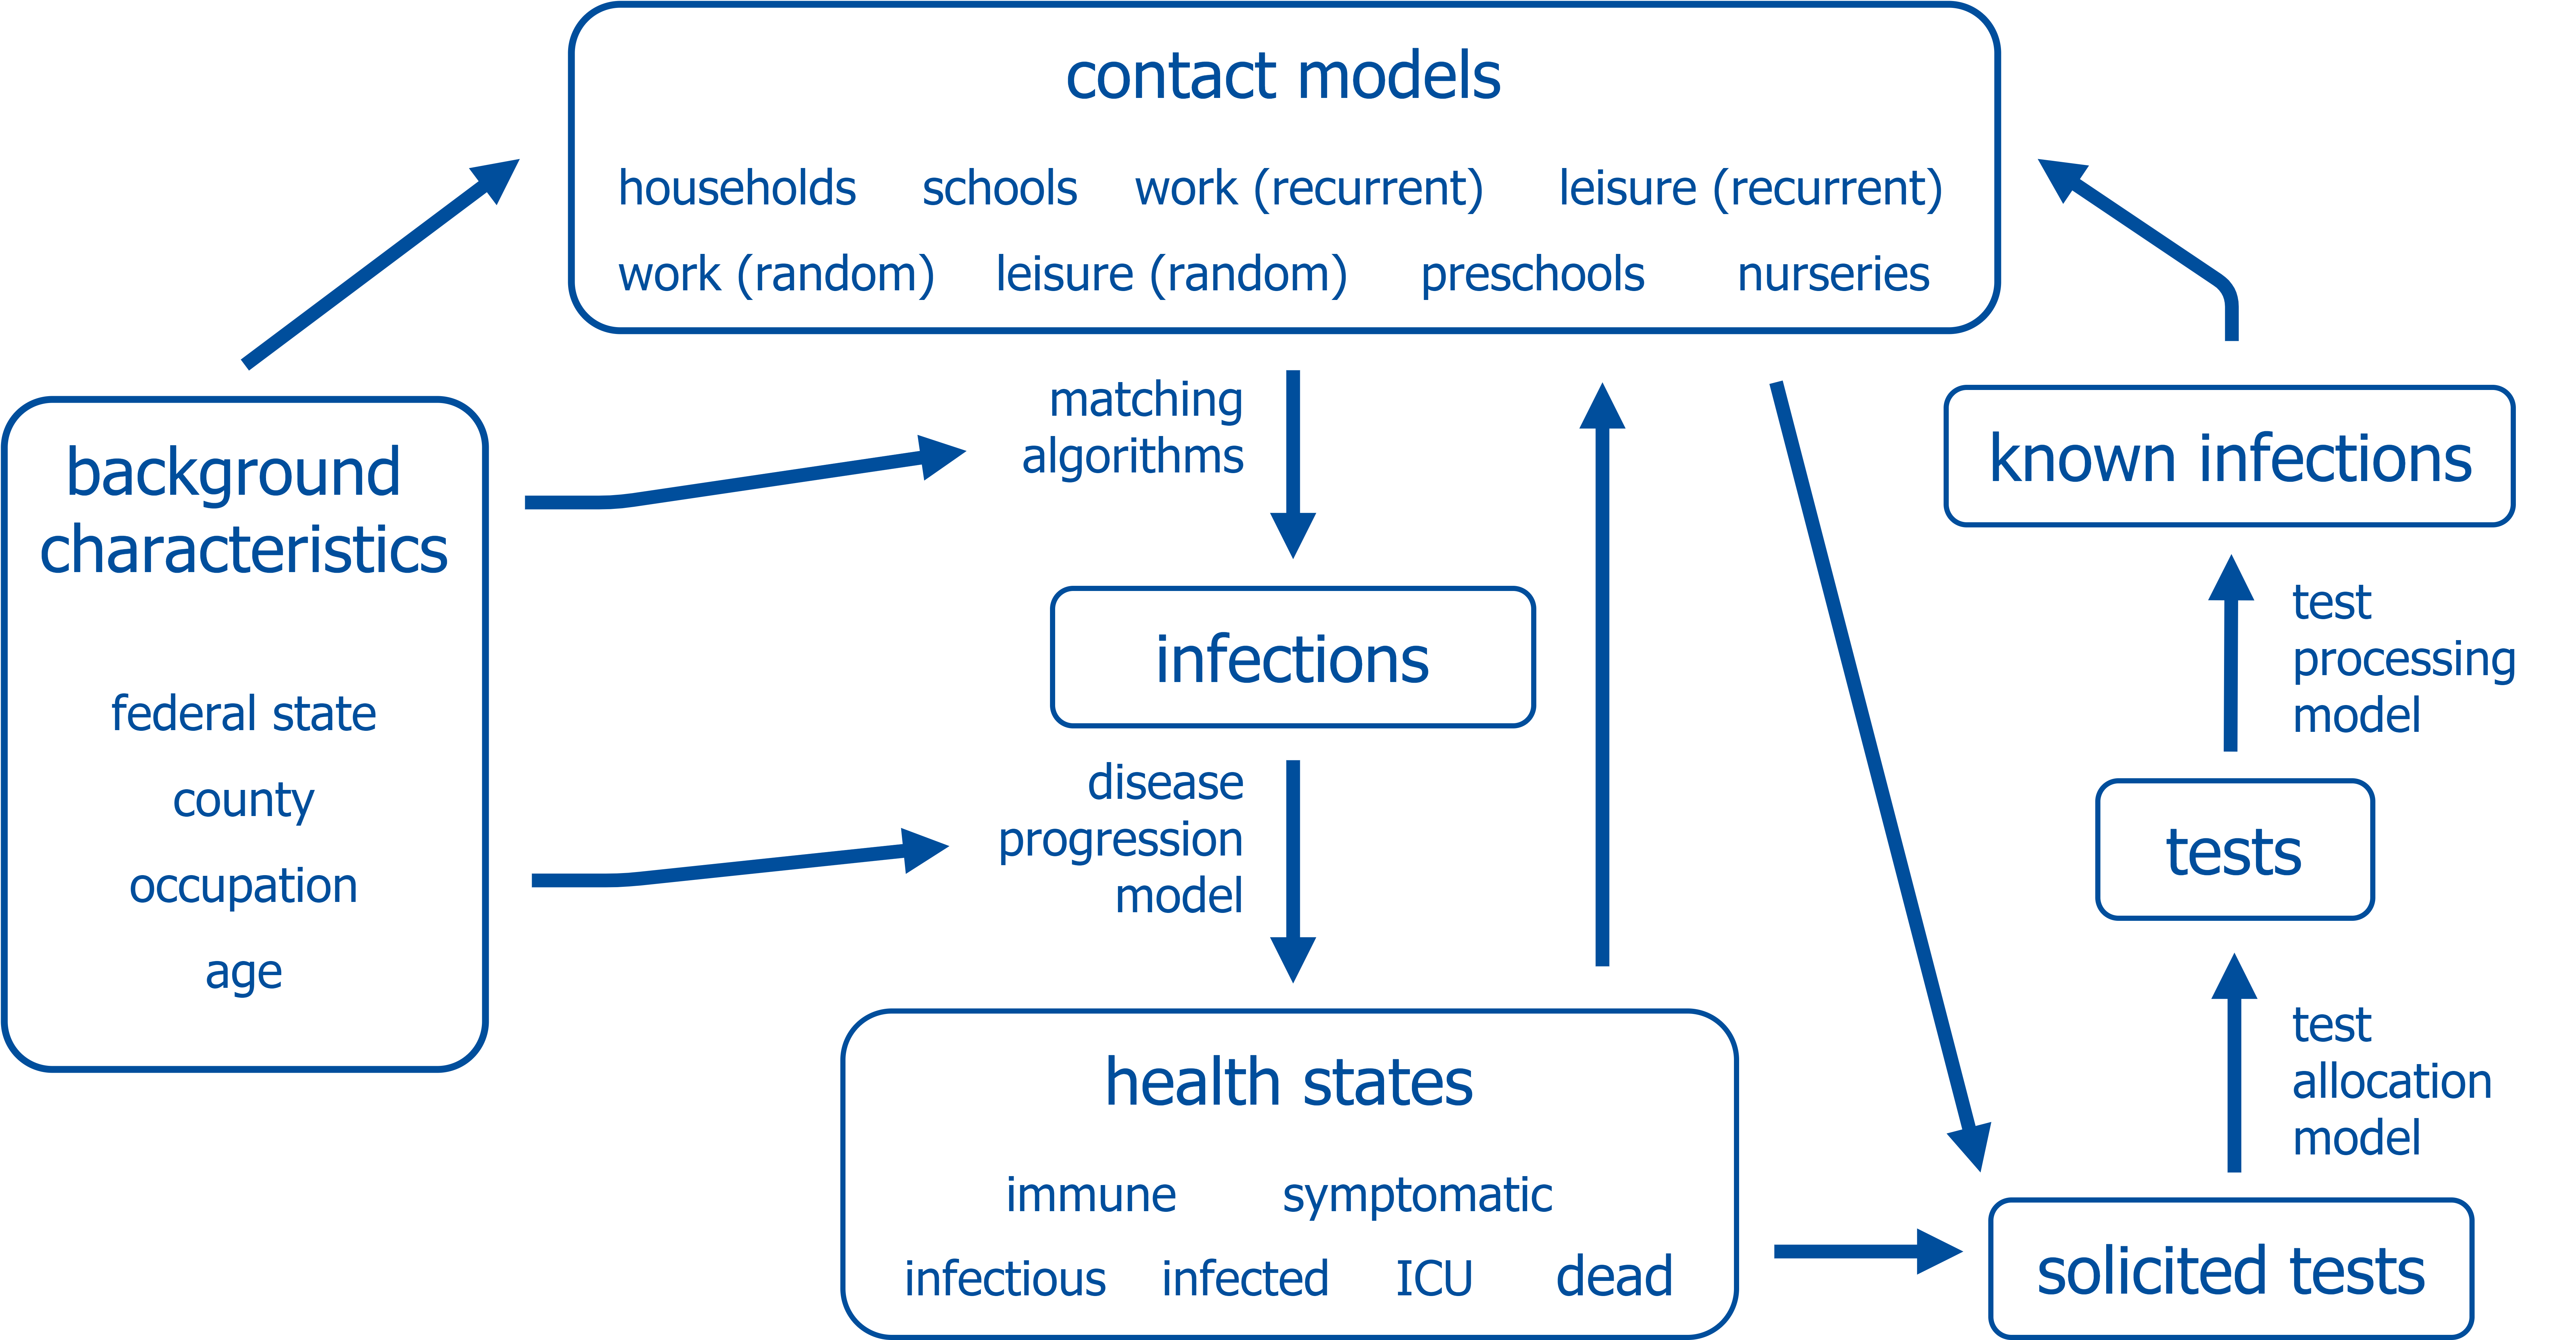
\includegraphics[width=0.7\textwidth]{../figures/model_detailed.png}
    \caption{Simplified graph of the model}
    \label{fig:model_graph}
\end{figure}

The background characteristics include age, county and occupation of each simulated individual. Contact models are functions that map individual characteristics into a predicted number of contacts. Currently we distinguish between eight types of contact models which are all listed in Figure~\ref{fig:model_graph}: households, recurrent and random work contacts, recurrent and random leisure contacts, and nursery, preschool, and school contacts.

The predicted number of contacts is translated into infections by a matching algorithm. There are different matching algorithms for recurrent contacts (e.g. classmates, family members) and non-recurrent contacts (e.g. clients, contacts in supermarkets). The infection probability can differ for each contact type. All types of contacts can be assortative with respect to geographic and demographic characteristics.

Once a person is infected, the disease progresses in a fairly standard way which is also depicted in Figure~\ref{fig:course_of_disease}. Asymptomatic cases and cases with mild symptoms are infectious for some time and recover eventually. Cases with severe symptoms additionally require hospitalization and lead to either recovery or death.

There are two possible ways to enable testing for Covid-19 in the model. The first way allows to specify the ratio of known to unknown infections for each day. A random sample of all newly infected individuals will then receive a test result in the following days. The second approach consists of three steps. First, individuals demand a test because they, e.g., experience symptoms. Secondly, tests are allocated to individuals while respecting governmental access restrictions to test. Thirdly, depending of the capacities of laboratories, tests are processed for some time until the individual receives her test result.

In addition, people who have symptoms, received a positive test, or had a risk contact can reduce their number of contacts across all contact types endogenously.

The model makes it very simple to translate policies into model quantities. For example, school closures imply the complete suspension of school contacts. A strict lockdown implies shutting down work contacts of all people who are not employed in a systemically relevant sector. It is also possible to have more sophisticated policies that condition the number of contacts on observable characteristics, risk contacts or health states.

Another key advantage of the model is that the number of contacts an individual has of each contact type can be calibrated from publicly available data \citep{Mossong2008}. This in turn allows us to estimate policy-invariant infection probabilities from time series of infection and death rates using the method of simulated moments \citep{McFadden1989}. Since the infection probabilities are time-invariant, data collected since the beginning of the pandemic can be used for estimation. Moreover, since we can model the testing strategies that were in place at each point in time, we can correct the estimates for the fact that not all infections are observed.

Last but not least, performing simulations whose starting point is set amidst the pandemic requires special adjustments to arrive at a realistic distribution of courses of diseases. We solve the initial conditions problem by matching reported infections to individuals in our data while also correcting for reporting lag and undetected cases.

In the following sections we describe each of the model components in more detail.
